\section{Раработка программного обеспечения}

\subsection{Разработка серверной части}

Структура приложения, написанного на фреймворке Django представляет собой набор отдельных приложений, выполняющих отдельные функции.
Каждое приложение вклбчает в себя:
\begin{itemize}
    \item models.py - файл, содержащий представление моделей базы данных;
    \item migrations/ - папка, хранящая миграции моделей;
    \item serialzers.py - файл, содержащий представления входных/выходных данных сервера;
    \item views.py - файл, содержащий контроллеры, обрабатывающие запросы;
    \item utils.py - файл, содержащий вспомогательные функции приложения, например сервисы обращения к третьим приложения;
    \item tasks.py - файл, содержищий асинхронные-задачи данного приложения, которые взаимодействуют с моделями это приложения, либо логически относятся к нему;
    \item tests.py - файл, содержащий тесты к контроллерам;
    \item factories.py - файл, содержащий фабрики для генерации данных для тестов;
    \item permissions.py - файл, содержащий пользовательские разрешения для запросов;
    \item signals.py - файл, содержащий сигналы для моделей БД;
    \item admin.py - файл, содержаший модели представления и модификации сайта администратора;
    \item urls.py - файл, содержищий связи между контроллерами и url-адресами.
\end{itemize}

Хоть Django фреймворк и предоставляет готовую структуру для написания веб-приложения, однако в каждом проекте присутствуют утилиты, нужные в независимости от приложения.
К таким утилитам относятся работы со структурами данных, работа с изображениями и интернализацией, миксины для контроллеров, сериализаторов либо тестов и тд.
Для таких утилит на уровне приложений была создана отдельная папка <<utils>>, содержащая модули python, разбитые по категориям:
\begin{itemize}
    \item strings.py - файл, содержащий утилиты для работы со строками;
    \item tests.py - папка, содержащий утилиты для работы с тестами;
    \item constants.py - файл, содержащий константы приложения;
    \item mixins.py - файл, содержащий миксины для сериализаторов и контроллеров;
    \item images.py - файл, содержащий утилиты для работы с изображениями;
    \item i18l.py - файл, содержащий утилиты для рабоыт с интернализацией;
    \item models.py - файл, содержащий утилиты для рабоыт с моделями.
\end{itemize}

Для предоставления возможности масштабирования системы была выбрана плоская структура конечных точек HTTP[19].
Данная структура характеризуется большим объемом мелких конечных точек, отвечающих за отдельные сущность.
Одновременно минусом и плюсом данной структуры является, как оговаривалось раньше, возможность получения конкретных объектов базы данных по средством отдельных конечных точек.
Таким образом, например, для получения всех данных о пользователе, клиент должен будеть послать несколько запросов к серверу.
Данная архитектура увеличивает количество запросов к серверу, однако сложно представить, что на одной странице клиента будут отображены все данные о пользователе.
И при нескольких конечных точках возможно, при ее необходимости, закгрузка данных в фоне.

На основании выбора плоской архитектуры к организации программного интерфейса к серверной части приложения были реализованы приложения: Auth, Users, Goods, Payments, Orders, Addresses (таблица 4.1).
Итоговая структура проекта представлена на рисунке \ref{back:struct}.

\begin{figure}[h!]
    \begin{subfigure}[b]{0.3\textwidth}
    \centering
    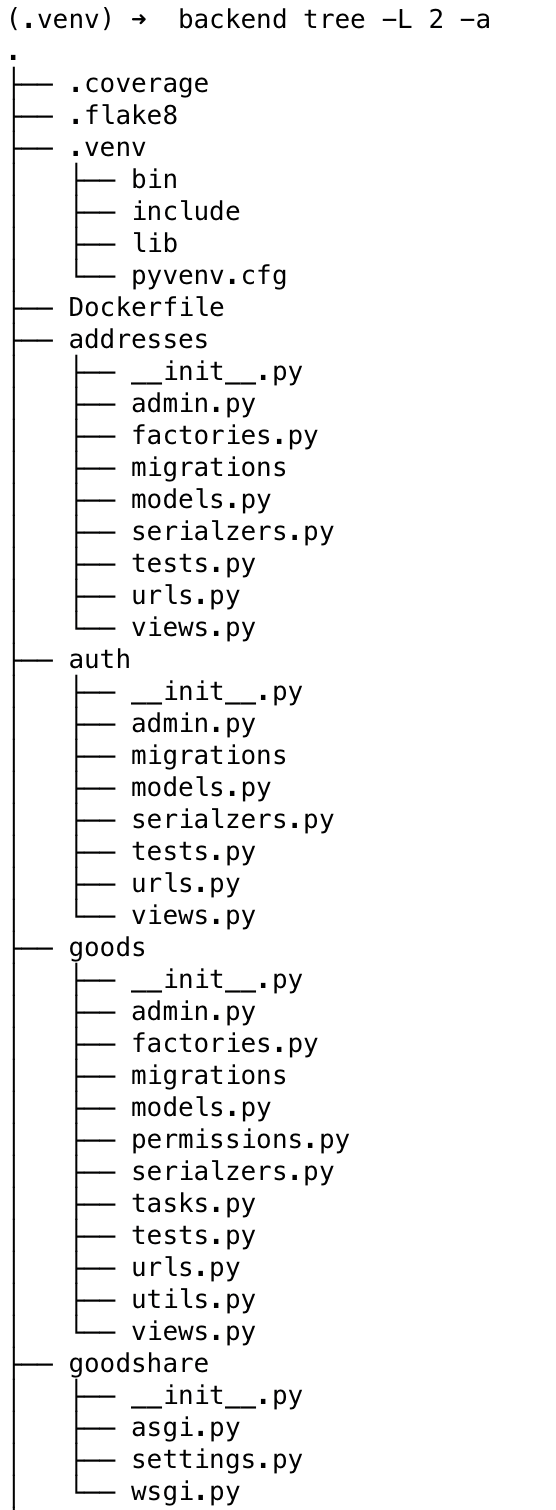
\includegraphics[scale=0.8]{structure_1.png}
    \caption{}
    \end{subfigure}
    \begin{subfigure}[b]{0.3\textwidth}
    \centering
    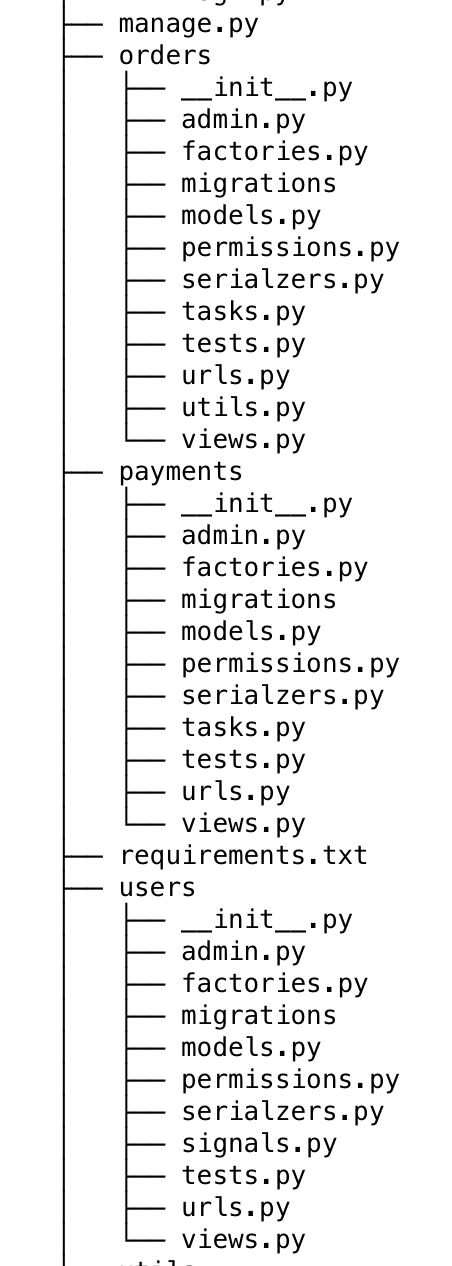
\includegraphics[scale=0.8]{structure_2.png}
    \caption{}
    \end{subfigure}
    \begin{subfigure}[b]{0.3\textwidth}
    \centering
    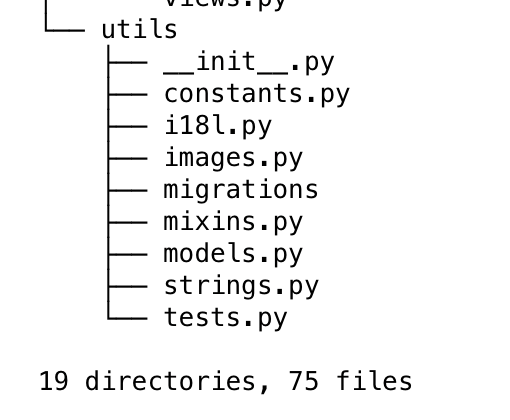
\includegraphics[scale=0.8]{structure_3.png}
    \caption{}
    \end{subfigure}
    \caption{ Структура серверной части приложения }
    \label{back:struct}
\end{figure}

\begin{table}
    \caption{Приложения серверной части}
    \begin{tabular}{ | l | p{6cm} | }
        \hline
        Название приложения & Выполняющие функции \\ \hline
        Auth & Отвечает за процесс авторизации пользователя в системе \\ \hline
        Users & Отвечает за манипуляции с пользовательскими данными \\ \hline
        Goods & Отвечает за доступ к товарам и взаимодействия с ними \\ \hline
        Payments & Хранения сохранненых данных для оплаты пользователя\\ \hline
        Orders & Хранения и соверщение заказов пользователя \\ \hline
        Addresses & Хранения адресов оплаты пользователя \\ \hline
    \end{tabular}
\end{table}

\subsubsection{Разработка моделей приложения}\hfill

Модель является единственным источником информации о данных.
Она содержит основные поля и поведение данных, которые в ней хранятся.
Как правило, каждая модель отображается в одну таблицу базы данных.
Для примера в листинге 4.1 будет представлен определение модели пользователя.

Листинг 4.1 – Определениние модели User
\begin{lstlisting}

    class User(AbstractUser):
        class Meta:
            ordering = ['-created_at']

        id = models.UUIDField(primary_key=True, default=uuid.uuid4, editable=False)
        name = models.CharField(max_length=128, null=True, blank=True)
        phone = PhoneNumberField(null=False, blank=False, db_index=True, unique=True)
        email = models.CharField(max_length=128, null=True, blank=True)
        fcm_token = models.CharField(max_length=128, null=True, blank=True)
        created_at = models.DateTimeField(auto_now_add=True, db_index=True)

        USERNAME_FIELD = 'phone'

        blocked_users = models.ManyToManyField(
            'users.User',
            related_name='blocked_by',
            blank=True,
        )

        is_blocked = models.BooleanField(default=False)

        def __str__(self):
            return self.get_full_name() or self.get_username()
\end{lstlisting}

Согласно сформулированным требованиям к ПО, пользователь должен иметь аватар.
На примере определения модели аватара пользователя(см листинг 4.2) будет представлено отношение модели <<UserAvatar>> к <<User>>.

Листинг 4.2 – Определениние модели UserAvatar
\begin{lstlisting}
    class UserAvatar(models.Model):
        class Meta:
            ordering = ('ordering',)

        ALLOWED_PHOTO_EXTENSIONS = ['png', 'jpeg', 'webp', 'jpg', 'jpe']
        id = models.UUIDField(primary_key=True, default=uuid.uuid4, editable=False)
        user = models.ForeignKey(
            'users.User', on_delete=models.CASCADE, related_name='images', limit_choices_to=10
        )
        url = models.CharField(max_length=10, blank=True, null=True)

        @property
        def image_path_prefix(self):
            return f'{self.user.pk}'

        def save(self, *args, **kwargs):
            if not self.extension:
                self.extension = self.url.split('.')[-1].lower()

            if self.extension not in self.ALLOWED_PHOTO_EXTENSIONS:
                raise Exception('The photo format %s is not allowed' % self.extension)

            super(UserImage, self).save(*args, **kwargs)

\end{lstlisting}

После определения модели, нужно сообщить Django, что о намерении использовать эти модели.
Для этого необходимо добавить приложение, в котором реализована данная модель в массив <<INSTALLED\_APPS>> в конфигурациооном файле проекта.


\subsubsection{Разработка сериализаторов приложения}\hfill

Модели Django интуитивно представляют данные, хранящиеся в базе, но API должен передавать информацию в менее сложной структуре.
Хотя данные будут представлены как экземпляры классов Model, их необходимо перевести в формат JSON для передачи через API.

Сериализатор DRF производит это преобразование.
Когда пользователь передает информацию (например, создание нового экземпляра) через API, сериализатор берет данные, проверяет их и преобразует в нечто, что Django может сложить в экземпляр модели.
Аналогичным образом, когда пользователь обращается к информации через API, соответствующие экземпляры передаются в сериализатор, который преобразовывает их в формат, который может быть легко передан пользователю как JSON.

Наиболее распространенной формой, которую принимает сериализатор DRF, является тот, который привязан непосредственно к модели Django
Код сериализатор представлен в листинге 4.3 ниже на примере сериализатора для модели Good.

Листинг 4.3 – Сериализатор модели Good
\begin{lstlisting}
    class GoodSerializer(serializers.ModelSerializer):
        images = GoodImageSerializer(many=True, required=False)
        class Meta:
            model = Good
            fields = (
                'name',
                'condition',
                'description',
                'can_be_purchased',
                'price_per_hour',
                'price_per_day',
                'own_delivery',
                'images',
            )
\end{lstlisting}

В сериализаторе, для модели Good был использован вложеннный сериализатор для модели GoodImage.
Настройки fields позволяют точно указать, какие поля доступны этому сериализатору.
В качестве альтернативы, может быть установлен exclude вместо fields, которое будет включать все поля модели, кроме тех, которые указаны в exclude.

\subsubsection{Разработка представлений приложения}\hfill

Сериализатор анализирует информацию в обоих направлениях (чтение и запись), тогда как ViewSet - это тот код, в котором определены доступные операции.
Наиболее распространенным ViewSet является ModelViewSet, который имеет следующие встроенные операции:
\begin{itemize}
    \item Создание экземпляра: create ();
    \item Получение / чтение экземпляра: retrieve ();
    \item Обновление экземпляра (все или только выбранные поля): update () или partial\_update ();
    \item Уничтожение / Удаление экземпляра: destroy ();
    \item Список экземпляров (с разбивкой по страницам по умолчанию): list ().
\end{itemize}

Каждая из этих функций может быть переопределена, если требуется другое поведение, но стандартная функциональность работает с минимальным кодом (см листинг 4.4).

Листинг 4.4 – Представление модели Address
\begin{lstlisting}
    class AddressesViewSet(viewsets.ModelViewSet):
        permission_classes = [permissions.IsAuthenticated]
        serializer_class = serializers.AddressSerializer
        queryset = models.Address.objects.all()
\end{lstlisting}

\subsubsection{Программный интерфейс серверной части}\hfill

На основании функциональных требований в каждом приложении были реализованы API конечных точек HTTP-запросов (таблицы 4.2-4.7).

\begin{table}
    \caption{Приложение Auth, базовый url адрес конечных точек <</auth>>}
    \begin{tabular}{ | p{3cm} | p{4cm} | p{3cm} | p{3cm} | }
        \hline
        url-адрес запроса / метод запроса & входные данные & выходные данные  & описание \\ \hline
    /verify POST  & phone - номер телефона, token - токен, выданные firebase, после вводна OTP кода & token - токен авторизации пользователя для осузествления запросов к серверу & С помощью данного запроса пользователь может авторизироваться в приложении с помощью токена \\ \hline
    \end{tabular}
\end{table}

\begin{table}
    \caption{Приложение Users, базовый url адрес конечных точек <</users>>}
    \begin{tabular}{ | p{3cm} | p{4cm} | p{3cm} | p{3cm} | }
        \hline
        url-адрес запроса / метод запроса & входные данные & выходные данные  & описание \\ \hline
        / POST & name - ФИО пользователя, photo - фото пользователя & созданная модель пользователя & создание пользователя в системе \\ \hline
        / PUT & name - ФИО пользователя, photo - фото пользователя, email - электронная почта пользователя & обновленная модель пользователя & обновление данных пользователя \\ \hline
        /ID/review POST & text - текст отзыва, mark - оценка пользователя & & создание отзыва о пользователе \\ \hline
        / GET & & получение информации о пользователе \\ \hline
    \end{tabular}
\end{table}

\begin{table}
    \caption{Приложение Addresses, базовый url адрес конечных точек <</addresses>>}
    \begin{tabular}{ | p{3cm} | p{4cm} | p{3cm} | p{3cm} | }
        \hline
        url-адрес запроса / метод запроса & входные данные & выходные данные  & описание \\ \hline
        / POST & city - город получателя, street - улица получателя, building - номер здания получателя, appartament - номер квартиры получателя & созданная модель адреса & создания адреса доставки пользователя \\ \hline
        /ID PUT & city - город получателя, street - улица получателя, building - номер здания получателя, appartament - номер квартиры получателя & обновленная модель адреса & обновление адреса доставки пользователя \\ \hline
        /ID DELETE & & & удаление адреса доставки пользователя \\ \hline
        / GET & & & получение всех сохраенных записей адресов \\ \hline
    \end{tabular}
\end{table}

\begin{table}
    \caption{Приложение Payments, базовый url адрес конечных точек <</payments>>}
    \begin{tabular}{ | p{3cm} | p{4cm} | p{3cm} | p{3cm} | }
        \hline
        url-адрес запроса / метод запроса & входные данные & выходные данные  & описание \\ \hline
        / POST & card\_number - номер карты пользователя, cvv\_code - cvv-код карты, date\_expire - срок годности карты, cardholder\_name - имя держателя карты & созданная модель оплаты & создание модели оплаты пользователя \\ \hline
        /ID PUT & card\_number - номер карты пользователя, cvv\_code - cvv-код карты, date\_expire - срок годности карты, cardholder\_name - имя держателя карты & обновленная модель оплаты & обновление модели оплаты пользователя \\ \hline
        /ID DELETE & & & удаление модели оплаты \\ \hline
        / GET & & & получение всех сохраенных записей оплат \\ \hline
    \end{tabular}
\end{table}

\begin{table}
    \caption{Приложение Goods, базовый url адрес конечных точек <</goods>>}
    \begin{tabular}{ | p{3cm} | p{4cm} | p{3cm} | p{3cm} | }
        \hline
        url-адрес запроса / метод запроса & входные данные & выходные данные  & описание \\ \hline
        /add POST & name - название товара, condition - состояние товара, description - описание товара, can\_be\_purchased - возможность выкупа товара, price\_per\_hour - цена аренды товара за час, price\_per\_day - цена аренды товара за сутки, own\_deliver - возможность доставки товара арендадателем & созданная модель товара & создания товара \\ \hline
        /ID PUT & name - название товара, condition - состояние товара, description - описание товара, can\_be\_purchased - возможность выкупа товара, price\_per\_hour - цена аренды товара за час, price\_per\_day - цена аренды товара за сутки, own\_deliver - возможность доставки товара арендадателем & обновленная модель товара & обновление информации о товаре \\ \hline
        /ID DELETE & & & удаление товара \\ \hline
        /ID/add-to-basket PUT &  & & добавление товара в корзину \\ \hline
        /ID/remove-from-basket PUT & & & удаление товара из корзины \\ \hline
        /?page=PAGE GET & PAGE - страница поисков & список моделей товаров & получить все товары \\ \hline
        /?page=PAGE \&XX=YY GET & PAGE - страница поисков, XX=элемент фильтрации, YY -  значение XX фильтра & список моделей товаров & получить все товары \\ \hline
    \end{tabular}
\end{table}

\begin{table}
    \caption{Приложение Orders, базовый url адрес конечных точек <</orders>>}
    \begin{tabular}{ | p{3cm} | p{4cm} | p{3cm} | p{3cm} | }
        \hline
        / POST & start\_use\_date - дата начала пользования, end\_use\_date - дата окончания пользования, payment - выбор оплаты, address - выбор адреса доставки & модель заказа & создание заказа \\ \hline
        /ID/pay PUT & & & оплата товара; \\ \hline
        / GET & & список моделей заказов & получение списка заказов. \\ \hline
    \end{tabular}
\end{table}

\subsection{Разработка клиентской части}

Как было описано в разделе про проектирование клиентской части, в среде React приложений нет четко выработанной структуры приложений.
Однако основываясь на практиках написания React приложений была реализованна структура приложения, представленная на рисунке \ref{front:struct}.

Глобальное состояние приложения была разделено на несколько редьюсеров:
\begin{itemize}
    \item appReducer - котнролирует глобальное состояние приложение, а именно контроль отображения загрузчиков в приложении;
    \item authReducer - контролирует изменение и процесс аунтентификации пользователя;
    \item basketReducer - контролирует состояние корзины пользователя;
    \item checkoutReducer - контролирует процесс покупки товара;
    \item filterReducer - отвечает за фильтрацию товаров на экране поиска товаров;
    \item productReducer - отвечает за создание и изменения пользовательских продуктов;
    \item profileReducer - отвечает за состяние пользовательских данных;
    \item orderReducer - отвечает за состояние пользовательских заказов;
\end{itemize}

Соответственно каждому редьюсеру были созданы саги, экшены и константы, которые провоцируют приложению на осуществление запросов на сервер либо изменение состояния.

Компоненты приложения расположены в директориях <<components>> и <<views>> таким образом, что в директории <<components>> расположены глупые компоненты, представляющие репрезентационные компоненты.
А в дирректории <<views>> расположены как экраны приложения, так и компоненты-контейнеры.
\begin{figure}[h]
    \begin{subfigure}[b]{0.45\textwidth}
    \centering
    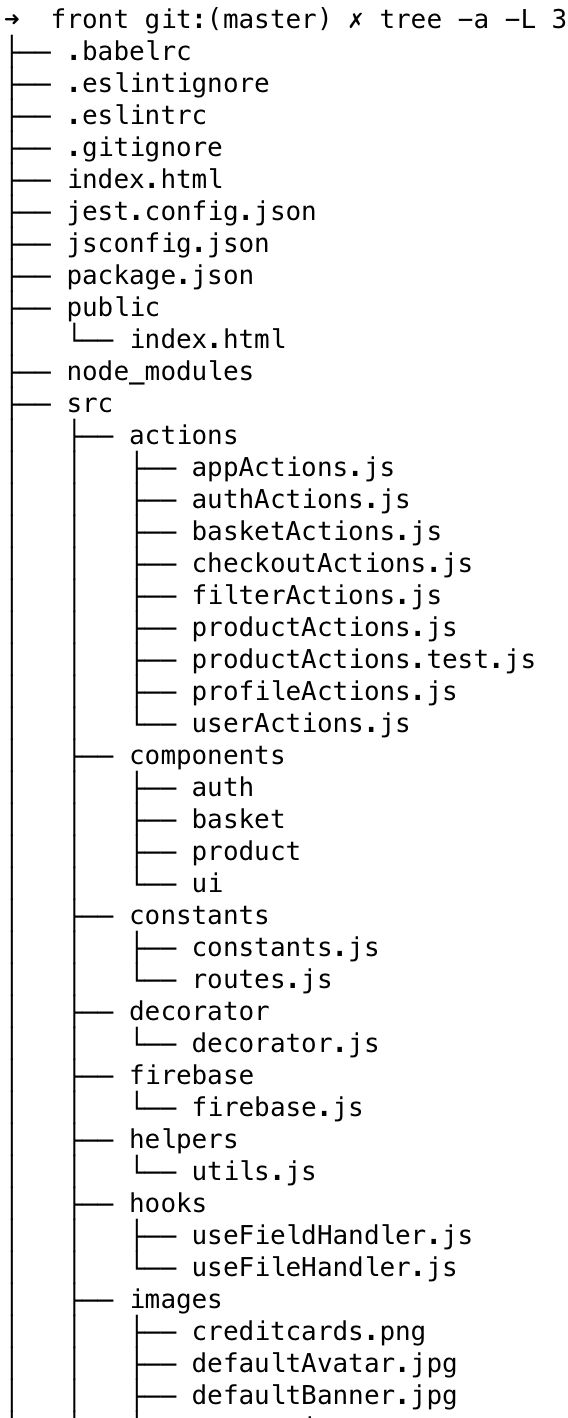
\includegraphics[scale=0.8]{front_structure_1.png}
    \caption{}
    \end{subfigure}
    \begin{subfigure}[b]{0.3\textwidth}
    \centering
    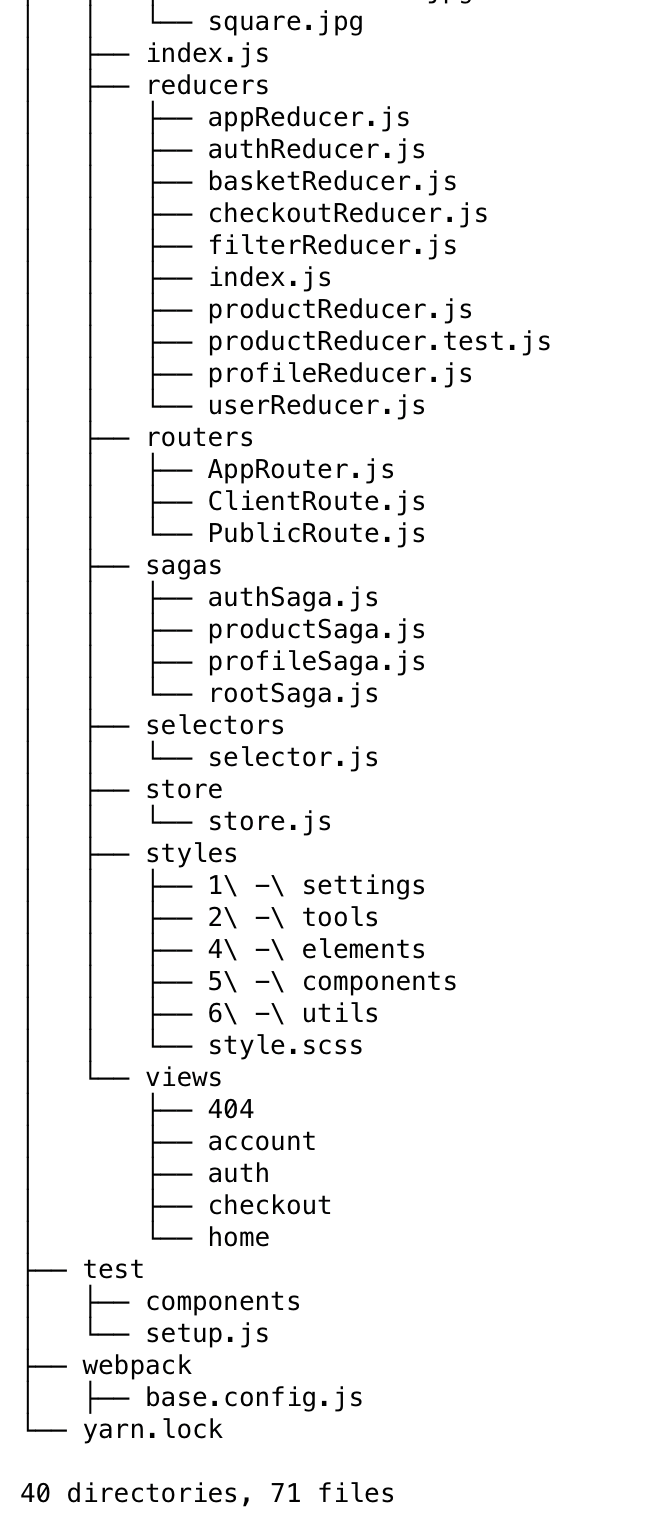
\includegraphics[scale=0.8]{front_structure_2.png}
    \caption{}
    \end{subfigure}
    \caption{ Структура клиентской части приложения }
    \label{front:struct}
\end{figure}

\subsubsection{Глобальное состояние приложения и асинхронные запросы}\hfill
Для начала стоит подчеркнуть, что Redux не имеет отношения к React.
Можно создавать Redux-приложения c помощью React, Angular, Ember, jQuery или обычного JavaScript.

Однако, Redux работает особенно хорошо с такими фреймворками, как React и Deku, потому что они позволяют описать UI как функцию состояния, и, кроме того, Redux умеет менять состояние (state) приложения в ответ на произошедшие экшены (actions).

React байндинг для Redux отделяют презентационные компоненты от компонент-контейнеров.
Такой подход может облегчить понимание приложения и упростить повторное использование компонентов.

Подход redux предполагает наличие 2х стоставляющих - reducer - функция изменения состояния приложения.
Обычно, это чистая функция, изменяющая свое состояние в зависимости от входных параметров - actions.
Action - представляет собой словарь с двумя полями: actionType  и payload.
В зависимости от actionType redux меняет одну из своих частей состояния.

В листинге 4.5-4.6 приведен пример reducer и actions к состоянию products.

Листинг 4.5 - Reducer состояния products
\begin{lstlisting}
    export default (state = {
    lastRefKey: null,
    total: 0,
    items: []
    }, action) => {
    switch (action.type) {
        case GET_PRODUCTS_SUCCESS:
        return {
            ...state,
            lastRefKey: action.payload.lastKey,
            total: action.payload.total,
            items: [...state.items, ...action.payload.products]
        };
        default:
        return state;
    }
    };
\end{lstlisting}

Листинг 4.6 - Actions состояния products
\begin{lstlisting}
    export const getProducts = lastRef => ({
    type: GET_PRODUCTS,
    payload: lastRef
    });

    export const getProductsSuccess = products => ({
    type: GET_PRODUCTS_SUCCESS,
    payload: products
    });

    export const cancelGetProducts = () => ({
    type: CANCEL_GET_PRODUCTS
    });

\end{lstlisting}

По умолчанию, экшены в Redux являются синхронными, что, является проблемой для приложения, которому нужно взаимодействовать с серверным API, или выполнять другие асинхронные действия.
Однако, Redux предоставляет нам такую штуку как middleware, которая стоит между диспатчом экшена и редюсером.
Существует две самые популярные middleware библиотеки для асинхронных экшенов в Redux, это — Redux Thunk и Redux Saga.
В данном проекте была выбрана библиотека redux-saga в виду того, что Sagas предлагает независимое место для обработки всех побочных эффектов.
А так же поставляется с множеством полезных вспомогательных функций о задачах.

В листинге 4.7 представлена сага, отвечающая ща манипуляции с аунтетификацией пользователя.

Листинг 4.7 - Сага состояния auth
\begin{lstlisting}
    function* handleError(e) {
    yield put(isAuthenticating(false));
    switch (e.code) {
        case 'auth/network-request-failed':
        yield put(setAuthStatus({ success: false, message: 'Network error has occured. Please try again.' }));
        break;
        default:
        yield put(setAuthStatus({ success: false, message: e.message }));
        break;
    }
    }

    function* authSaga({ type, payload }) {
    switch (type) {
        case SEND_CODE:
        try {
            const confirmationResult = yield call(firebase.sendCode, payload.phone, payload.appVerifier);
            yield put(sendCodeSuccess(confirmationResult));
        } catch (e) {
            yield handleError(e);
        }
        break;
        case VERIFY_CODE:
        try {
            const state = yield select();
            yield call(firebase.verifyCode, state.auth.confirmationResult, payload);
            yield put(isAuthenticating(false));
        } catch (e) {
            yield handleError(e);
        }
        break;
        case SIGNOUT:
        try {
            yield call(firebase.signOut);
            yield put(signOutSuccess());
            yield put(isAuthenticating(false));
            yield call(history.push, '/signin');
        } catch (e) {
            console.log(e);
        }
        break;
        default:
    }
    }

    export default authSaga;
\end{lstlisting}

Как можно увидеть выше, сага представляет собой reducer, который вместо того, чтобы изменять состояние приложения, вызывает асинхронные действия.

\subsubsection{Разработка интерфейса}\hfill

На примере компоненты Home (см листинг 4.8) будет продемонстрированно подключение Redux состояния и redux-saga к компоненту.
В данном проекте использовалась библиотека react-redux, которая позволяет с помощью хуков пользоваться redux в компоненте, без подключения ее через функцию connect.

Листинг 4.8 - Подключение компоненты Home к redux
\begin{lstlisting}
    import { useSelector, useDispatch } from 'react-redux';
    import { selectFilter } from 'selectors/selector';
    const { store } = useSelector(state => ({
        store: {
          productsLength: state.products.items.length,
          products: state.products.items,
          filter: state.filter,
          basket: state.basket,
          lastRefKey: state.products.lastRefKey,
          totalItems: state.products.total,
          isLoading: state.app.loading,
          filteredProducts: selectFilter(state.products.items, state.filter),
          requestStatus: state.app.requestStatus
        }
      }));

      const dispatch = useDispatch();
      const productListWrapper = useRef(null);

\end{lstlisting}


\subsection{Интеграция Firebase}
В данном проекте из платформы Firebase использовались 2 модуля:
\begin{itemize}
    \item Authentication;
    \item Messaging.
\end{itemize}

На серверной части интеграция с Firebase происходит с помощью пакета firebase-admin.
Для инициализации Firebase проекта на серверной части необходимо скачать сервисный файл с панели администратора на Firebase(см рисунок \ref{fire:admin}).

\begin{figure}[ht]
    \centering
    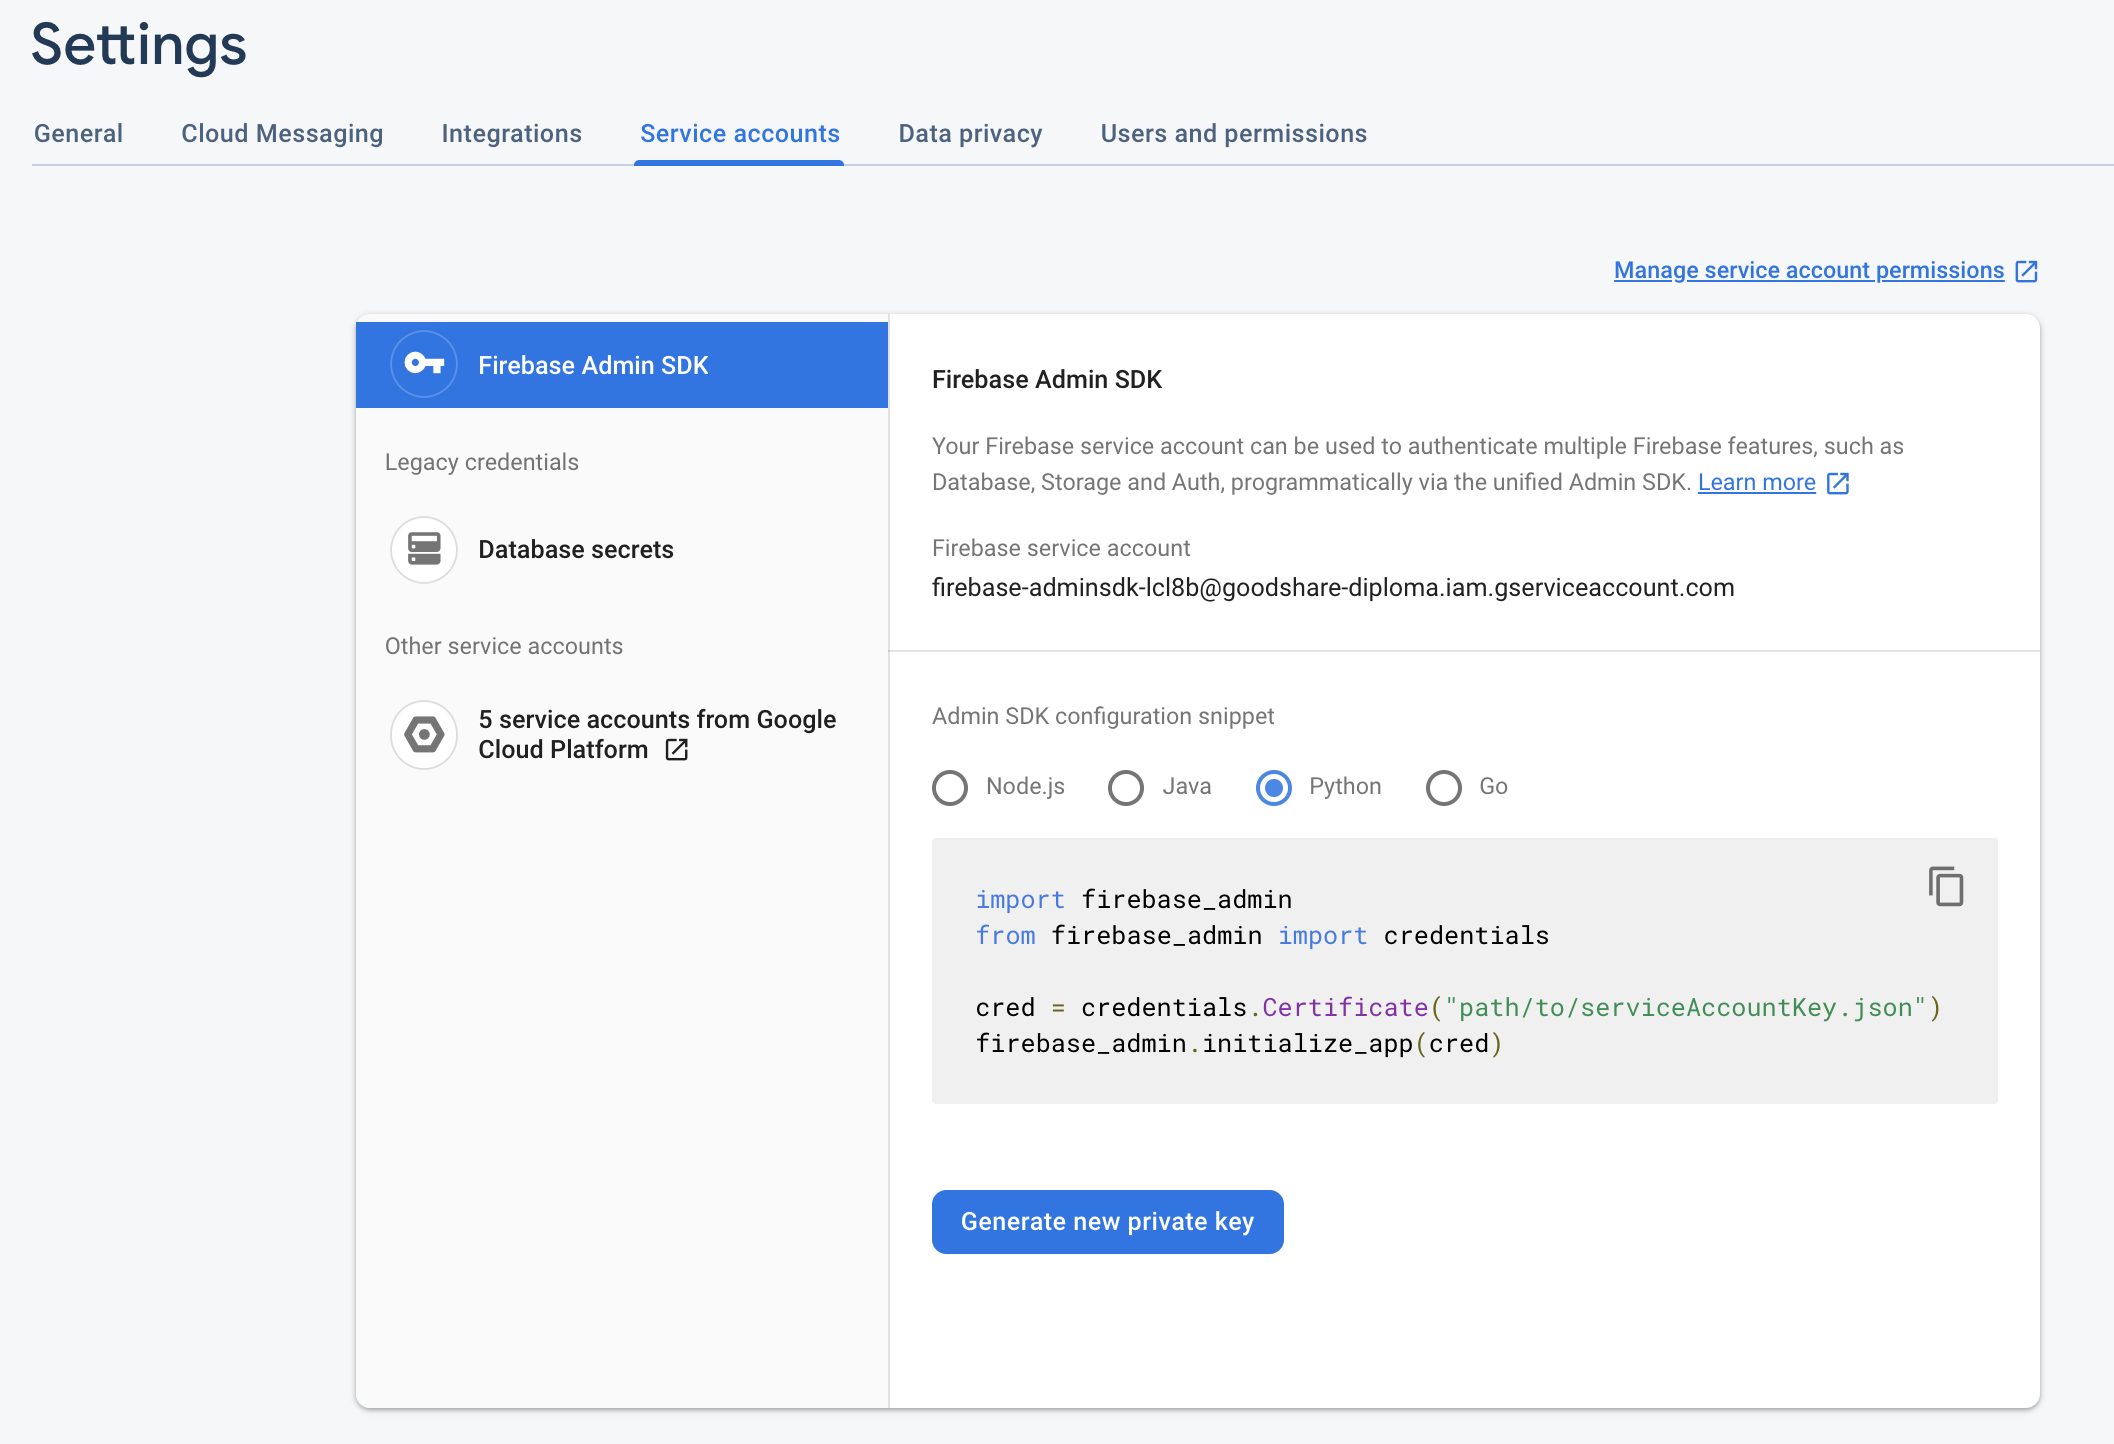
\includegraphics[scale=0.4]{service_file.png}
    \caption{ Графический интерфейс Firebase вкладки скачивания сервисного файла }
    \label{fire:admin}
\end{figure}

Далее данный файл используется для инициализации проекта (см листинг 4.9).

Листинг 4.9 – Инициализация Firebase на серверной части
\begin{lstlisting}
    import os

    import firebase_admin

    from firebase_admin import credentials

    firebase_admin.initialize_app(
        credentials.Certificate(
            os.environ["FIREBASE_SERVICE_FILE"]
        )
    )
\end{lstlisting}

После чего в разделах ниже будет добавлен и использован функционал данной библиотеки для реализации отправки уведомлений и организации аунтентификации по номеру телефона.


В целях соблюдения концепции <<Двенадцать факторов>>, а так же облегчения развертывания проекта, инициализация проекта клиентской части происходит с помощью переменных окруженя.
Как и для серверной части, данные доступа приложения можно получить в панели администратора Firebase.

Для того, чтобы облегчить процесс использования сервисов Firebase на клиентской части, был написан сервис Firebase(см листинг 4.10).

Листинг 4.10 – Инициализация Firebase на клиентской части
\begin{lstlisting}
    import app from 'firebase/app';

    const firebaseConfig = {
      apiKey: process.env.FIREBASE_API_KEY,
      authDomain: process.env.FIREBASE_AUTH_DOMAIN,
      databaseURL: process.env.FIREBASE_DB_URL,
      projectId: process.env.FIREBASE_PROJECT_ID,
      storageBucket: process.env.FIREBASE_STORAGE_BUCKET,
      messagingSenderId: process.env.FIREBASE_MSG_SENDER_ID,
      appId: process.env.FIREBASE_APP_ID,
      measurementId: process.env.MEASUREMENT_ID
    };

    class Firebase {
      constructor() {
        app.initializeApp(firebaseConfig);
      }

    }

    const firebase = new Firebase();

    export default firebase;

\end{lstlisting}

Сервис представляет собой синглтон, который предоставляет доступ к инициализированному приложению.
В разделах ниже в него будут добавлены необходимые функции.

\subsubsection{Использование Firebase Authentication}\hfill

Firebase обеспечивает службы серверной части, простые пакеты разработчика и готовые библиотеки интерфейса для аутентификации пользователей различных приложения на любых платформах.
На основе требований к ПО было принято решение использования модуля Firebase Authentication с провайдером аутентификации Phone Number.

В первую очередь был создан набор тестовых номеров телефонов, потому что при использовании одного и того же номера для аутентификации Firebase может блокировать этот номер на некоторое время.
Список созданных тестовых номеров представлен на рисунке \ref{fire:phones}.
\begin{figure}[ht]
    \centering
    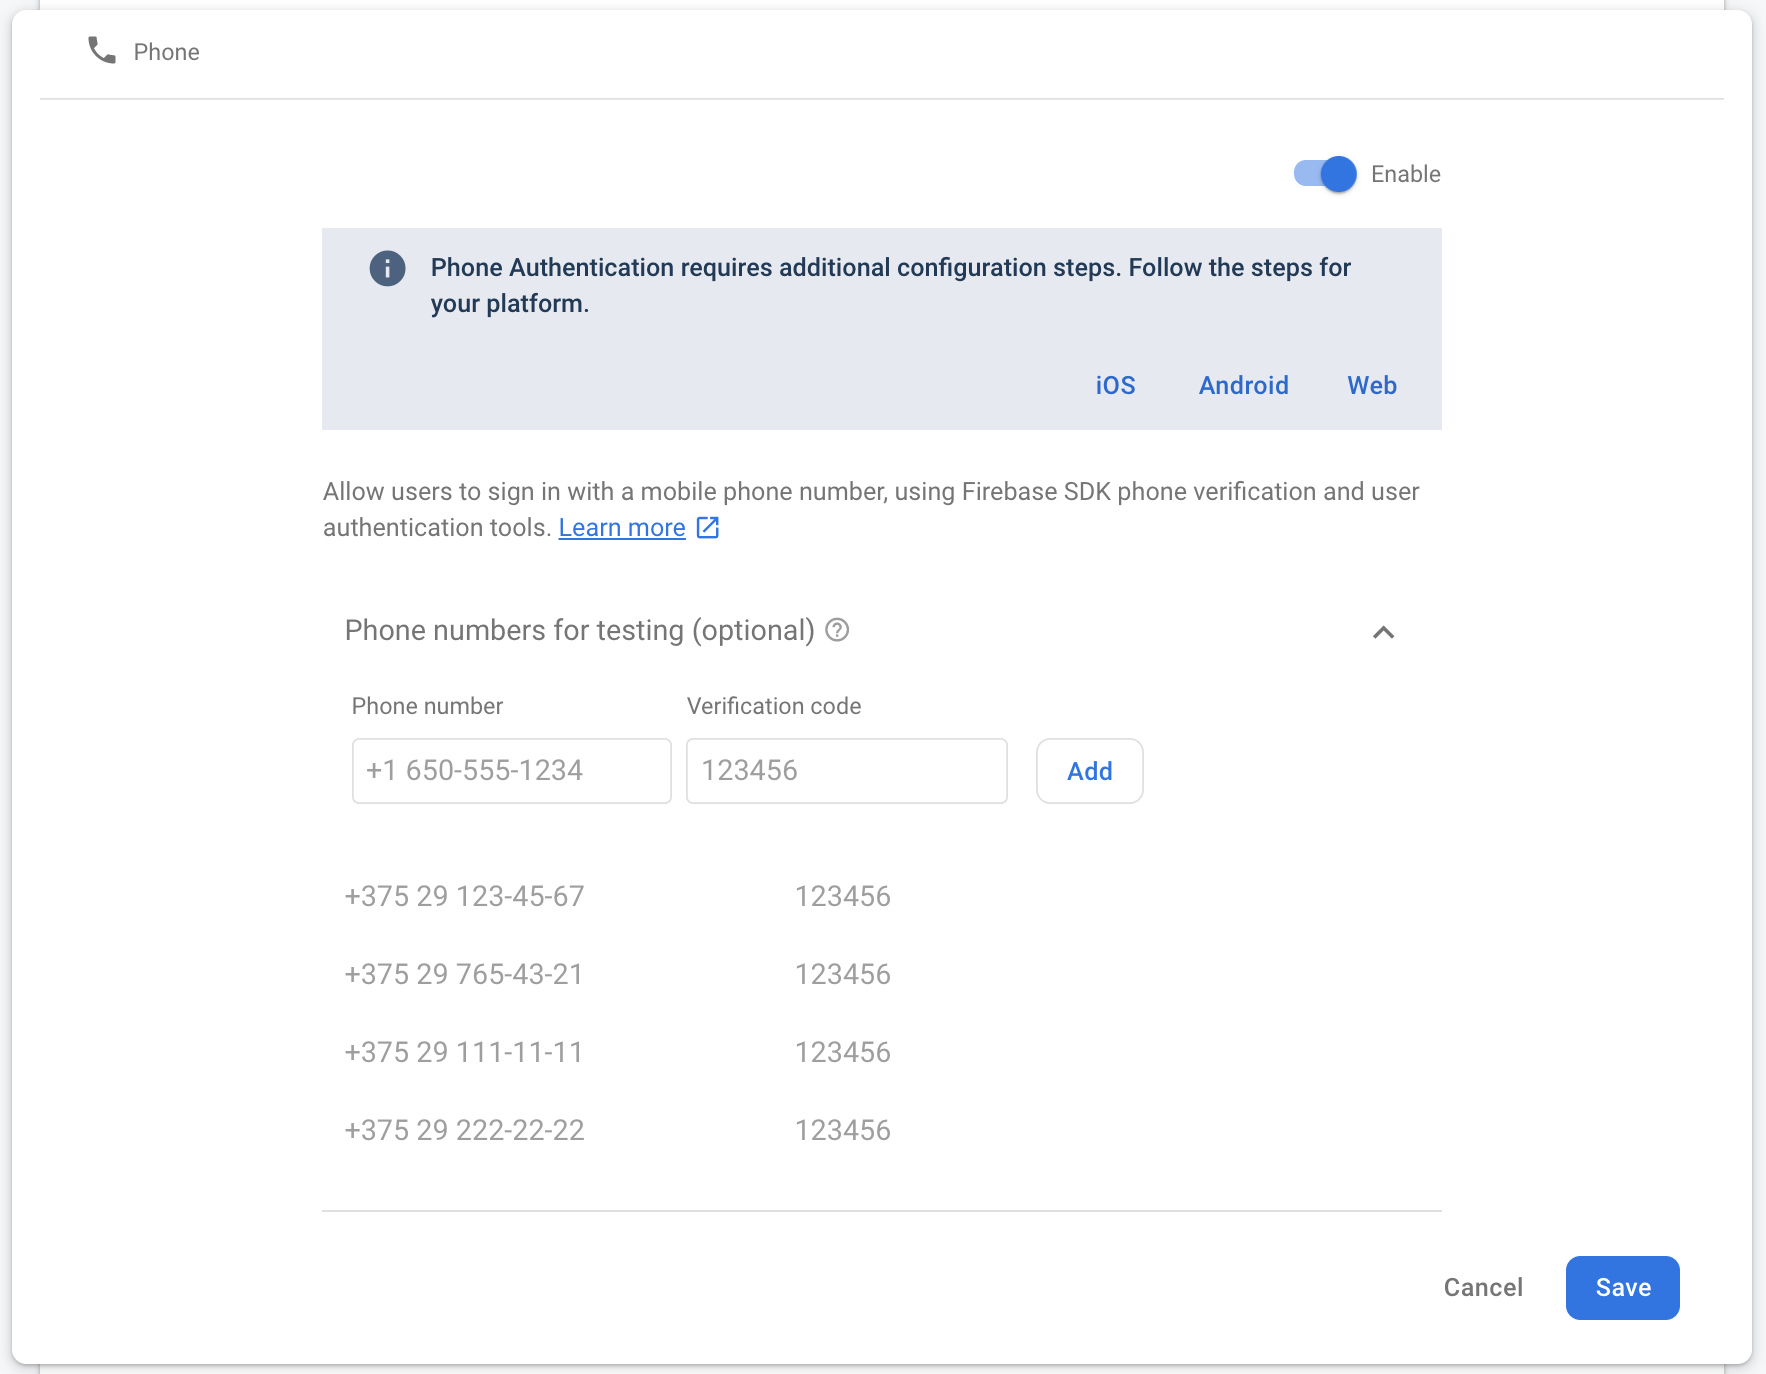
\includegraphics[scale=0.5]{firebase_phone_list.png}
    \caption{ Список используемые тестовых номеров телефонов }
    \label{fire:phones}
\end{figure}

После этого необходимо интегрировать использование аутентификации с помощью номера телефона на клиентскую часть.

Как было сказано выше, для удобного обращения к сервисам фаербейз был разработан модуль Firebase.
В нем были реализованы функции:
\begin{itemize}
    \item Выслать OTP-код на номер телефона;
    \item Проверить OTP-код;
\end{itemize}

Прежде чем войти в систему пользователей с их телефонов, необходимо настроить средство проверки рекапчи.
Firebase использует reCAPTCHA для предотвращения злоупотреблений.
Таким образов для интеграции Firebase Authentication с помощью номера телефона необходимо создать каптчу(см листинг 4.11).
И так же организовать проверку с помощью клиентской библиотеки Firebase(см листинг 4.12).


Листинг 4.11 – Интеграция reCAPTCHA в форму аунтентификации
\begin{lstlisting}
    useEffect(() => {
        window.recaptchaVerifier = new firebase.auth.RecaptchaVerifier('recaptcha-container', {
          callback: () => setCodeSent(true),
          size: 'invisible'
        });
      }, []);
\end{lstlisting}

Листинг 4.12 – Интеграция функционала для работы с аунтентификацией по номеру телефона
\begin{lstlisting}

class Firebase {
    constructor() {
      app.initializeApp(firebaseConfig);

      this.auth = app.auth();
    }

    sendCode = (phone, appVerifier) => this.auth.signInWithPhoneNumber(phone, appVerifier);

    verifyCode = (confirmationResult, code) => confirmationResult.confirm(code);

    signOut = () => this.auth.signOut();
  }

\end{lstlisting}

После успешной проверки OTP-кода Firebase генерирует IdToken, котрый представляет собой JWT токен.
Данный токер вместе с номером телефона отправляется на серверную часть для получения токена авторизации.

Для обработки процесса аунтентификации пользователя на серверной части была реализована проверка IdToken с помощью серверной библиотеки Firebase.


Был написан сериализатор(см листинг 4.13), который средствами серверной библиотеки Firebase распаковывает IdToken и проверяет, соответствие номера телефона запроса с номером телефона в токене.

Листинг 4.13 – Сериализатор проверки код и номера телефона
\begin{lstlisting}
from django.utils.translation import ugettext_lazy as _
from phonenumber_field.serializerfields import PhoneNumberField

from rest_framework import serializers, exceptions
from utils.firebase.helpers import get_id_token


class FireBaseIDTokenSerializer(serializers.Serializer):
    fcm_token = serializers.CharField(
        allow_null=True, max_length=200
        )
    phone_number = PhoneNumberField()
    verification_code = serializers.CharField()

    def validate_verification_code(self, value):
        try:
            decoded_token = get_id_token(value)
        except ValueError:
            raise exceptions.ValidationError(
                _("Token expired!"), code="token-expired"
            )
        except Exception:
            # TODO: Add logging
            raise exceptions.ValidationError(
                _("Invalid code!"), code="token-invalid"
            )
        return decoded_token

    def validate_phone_number(self, value):
        return value.as_e164

    def validate(self, attrs):
        decoded_token = attrs["verification_code"]
        if decoded_token["phone_number"] != attrs["phone_number"]:
            raise exceptions.ValidationError(
                _("Invalid combination of phone number and code!")
            )

        return attrs

\end{lstlisting}

При неуспешной обработке токена сервер возвращает 40X ответ клиентской части с описанием ошибки.
При успешной обработке токена сервер генерирует токен авторизации и возвращает его в ответе.

\subsubsection{Использование Firebase Messaging}\hfill

Firebase Cloud Messaging (FCM) - это кросс-платформенное решение для обмена сообщениями, которое позволяет  отправлять сообщения без каких-либо затрат.

На серверной части была написана утилита для отправки уведомлений как одному пользователю, так и многим (см листинг 4.14-4.16).


Листинг 4.14 – Функция создания конфигурационного файла для отправки уведомлений
\begin{lstlisting}
    def generate_push_configs(
        title: str = None, body: str = None, url: str = ""
        ) -> messaging.WebpushConfig:

    url_site = f"https://{os.environ["SSL_DOMAIN"]}"
    redirect_to = f"{url_site}/{url}" if url else None

    webpush_config = messaging.WebpushConfig(
        notification=messaging.WebpushNotification(
            title=title,
            body=body,
        ),
        fcm_options=messaging.WebpushFcmOptions(
            link=redirect_to
        )
    )
    return webpush_config
\end{lstlisting}

Листинг 4.15 – Отправка уведомления одному пользователю
\begin{lstlisting}
    def send_push(
        user_id: int, collection: str, title: str = None,
        body: str = None, url: str = ""
        ) -> None:
    token = User.objects.get(pk=user_id).fcm_token
    if not token:
        return

    webpush_config = generate_push_configs(title, body, url)

    message = messaging.Message(
        webpush=webpush_config,
        token=token
    )
    try:
        messaging.send(message)
    except messaging.ApiCallError as e:
        logging.debug(
            f"Could send push in firebase. Error: {e}"
            )
\end{lstlisting}

Листинг 4.16 – Отправка уведомления нескольким пользователям
\begin{lstlisting}
    def send_multiple_push(
        users_ids: list, collection: str, title: str = None,
        body: str = None, url: str = ""
        ) -> None:
    tokens = (
        User.objects
        .filter(pk__in=users_ids)
        .values_list("fcm_token", flat=True)
    )
    filtered_tokens = [token for token in tokens if token]

    webpush_config = generate_push_configs(title, body)

    multicast_message = messaging.MulticastMessage(
        tokens=filtered_tokens,
        webpush=webpush_config,
    )
    try:
        messaging.send_multicast(multicast_message)
    except messaging.ApiCallError as e:
        logging.debug(
            f"Could send multicast push in firebase. Error: {e}"
            )
\end{lstlisting}

Токен для отправки уведомлений обновляется при аутентификации пользователя в системе.
Во избежании ошибок при отправке уведомлений была добавлена проверка на наличие FCM токена у пользователя.

\subsection{Развертывание программного обеспечения}
В первую очередь стоит обратить внимание на то, что данный проект состоит из трех компонент:
\begin{itemize}
    \item Клиентское приложение;
    \item Серверное приложение;
    \item База данных.
\end{itemize}

При том изобилии компонент, которое у имеется, решением для разработки было использование docker-compose.
Таким образом был написан <<docker-compose.yml>> файл(см листинг 4.17).

Листинг 4.17 – Docker-compose файл
\begin{lstlisting}
    version: "3"

    services:
    db:
        image: postgres
        ports:
        - "5432:5432"
    django:
        build: ./backend
        command: bash -c 'python manage.py
        migrate && python manage.py runserver 0.0.0.0:8000'
        ports:
        - "8000:8000"
        depends_on:
        - db
    frontend:
        build: ./frontend
        command: npm start
        volumes:
        - ./frontend:/app/frontend
        ports:
        - "8000:8000"
\end{lstlisting}


Данный файл состоит соответственно из трех сервисов: клиентское приложние, серверное приложение и база данных.
Стоит обратить внимание, что серверное приложение не может быть запущено, пока не запущена база данных.
так же клиентское приложение не может быть запущено, пока не запущено серверное приложеие.
Во избежании увеличения размера файла было решено хранить переменные окружения в образах самих сервисов.

Далее были написаны файлы Dockerfile для клиентского и сервеного приложений(см листинг 4.18-4.19).


Листинг 4.18 – Dockerfile клиентского приложения
\begin{lstlisting}
    FROM node

    ENV PATH /node_modules/.bin:$PATH
    WORKDIR /usr/src/front

    COPY package.json ./
    COPY package-lock.json ./

    RUN npm install --silent
    RUN npm install react-scripts@3.4.1 -g --silent

    COPY . /usr/src/front/
\end{lstlisting}

Листинг 4.19 – Dockerfile серверного приложения
\begin{lstlisting}
    FROM python:3.8.0-alpine

    WORKDIR /usr/src/app

    ENV PYTHONDONTWRITEBYTECODE 1
    ENV PYTHONUNBUFFERED 1

    RUN pip install --upgrade pip
    COPY ./requirements.txt /usr/src/app/requirements.txt
    RUN pip install -r requirements.txt

    COPY . /usr/src/app/

\end{lstlisting}

Таким образом командой <<docker-compose up>> можно запустить проект.
